% \documentclass[aspectratio=169,notes]{beamer}
\documentclass[aspectratio=169]{beamer}
\usetheme[faculty=phil]{fibeamer}
\usepackage{polyglossia}
\setmainlanguage{english} %% main locale instead of `english`, you
%% can typeset the presentation in either Czech or Slovak,
%% respectively.
\setotherlanguages{russian} %% The additional keys allow
%%
%%   \begin{otherlanguage}{czech}   ... \end{otherlanguage}
%%   \begin{otherlanguage}{slovak}  ... \end{otherlanguage}
%%
%% These macros specify information about the presentation
\title[AGLA1]{Analytical Geometry and Linear Algebra I, Lab 14} %% that will be typeset on the
\subtitle{Quadric surfaces: Cone, Cylinder
\\ \    \\ \  
         } %% title page.
\author{Oleg Bulichev}
%% These additional packages are used within the document:
\usepackage{ragged2e}  % `\justifying` text
\usepackage{booktabs}  % Tables
\usepackage{tabularx}
\usepackage{tikz}      % Diagrams
\usetikzlibrary{calc, shapes, backgrounds}
\usepackage{amsmath, amssymb}
\usepackage{url}       % `\url`s
\usepackage{listings}  % Code listings
% \usepackage{subfigure}
\usepackage{floatrow}
\usepackage{subcaption}
\usepackage{mathtools}
\usepackage{todonotes}
\usepackage{fontspec}
\usepackage{multicol}
\usepackage{pdfpages}
\usepackage{wrapfig}
\usepackage{animate}
\usepackage{booktabs}
\usepackage{multirow}

\graphicspath{{resources/}}
\frenchspacing

\setbeamertemplate{caption}[numbered]
\usetikzlibrary{graphs}

% \usepackage[backend=biber,style=ieee,autocite=footnote]{biblatex}
% \addbibresource{biblio.bib}
% \DefineBibliographyStrings{english}{%
%   bibliography = {References},}

\newcommand{\oleg}[2][] {\todo[color=red, #1] {OLEG:\\ #2}}
\newcommand{\fbckg}[1]{\usebackgroundtemplate{\includegraphics[width=\paperwidth]{#1}}}%frame background

\usepackage[framemethod=TikZ]{mdframed}
\newcommand{\dbox}[1]{
\begin{mdframed}[roundcorner=3pt, backgroundcolor=yellow, linewidth=0]
\vspace{1mm}
{#1}
\vspace{1mm}
\end{mdframed}
}

\begin{document}
\setlength{\abovedisplayskip}{0pt}
\setlength{\belowdisplayskip}{0pt}
\setlength{\abovedisplayshortskip}{0pt}
\setlength{\belowdisplayshortskip}{0pt}

\fbckg{fibeamer/figs/title_page.png}
\frame[c]{\setcounter{framenumber}{0}
    \usebeamerfont{title}%
    \usebeamercolor[fg]{title}%
    \begin{minipage}[b][6.5\baselineskip][b]{\textwidth}%
        \textcolor{black}{\raggedright\inserttitle}
    \end{minipage}
    % \vskip-1.5\baselineskip

    \usebeamerfont{subtitle}%
    \usebeamercolor[fg]{framesubtitle}%
    \begin{minipage}[b][3\baselineskip][b]{\textwidth}
        \raggedright%
        \insertsubtitle%
    \end{minipage}
    \vskip.25\baselineskip
}
%   \frame[c]{\maketitle}

\fbckg{fibeamer/figs/common.png}

\note{\scriptsize \begin{itemize}
    \item \ 
\end{itemize}}


\begin{frame}[t]{Case studies of 2nd order curve equation (ENG)}
\framesubtitle{}
    \vspace{-0.6cm}
    \begin{figure}[H]
        \centering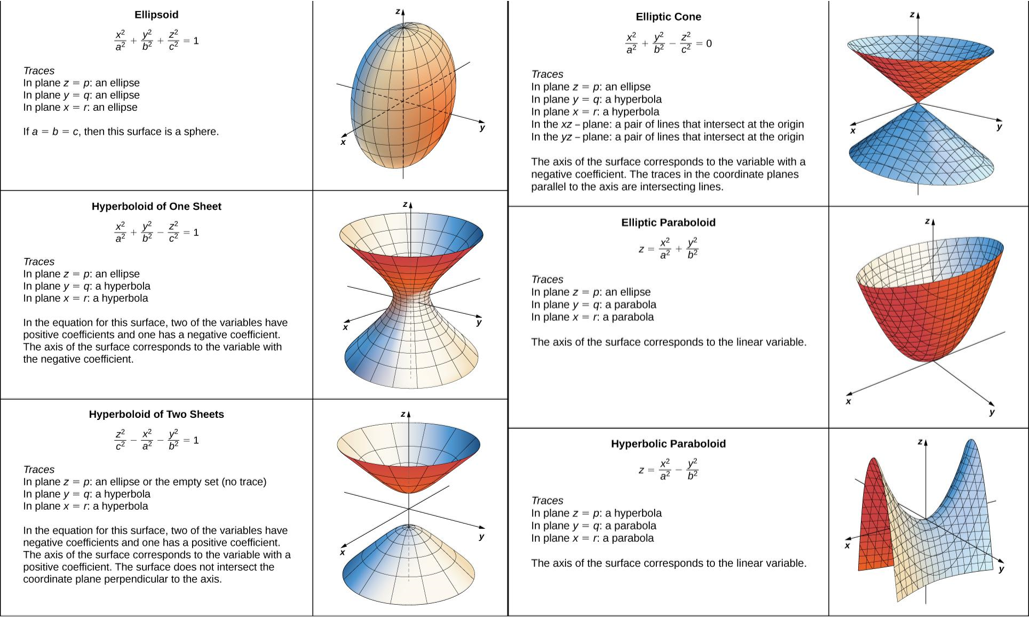
\includegraphics[height=6cm,width=1\textwidth,keepaspectratio]{curve_eq_eng.png}
        \label{fig:curve_eq_eng.png}
    \end{figure}
\end{frame}

\begin{frame}[t]{Case studies of 2nd order curve equation (RUS)}
    \framesubtitle{}
        \vspace{-0.6cm}
        \begin{figure}[H]
            \centering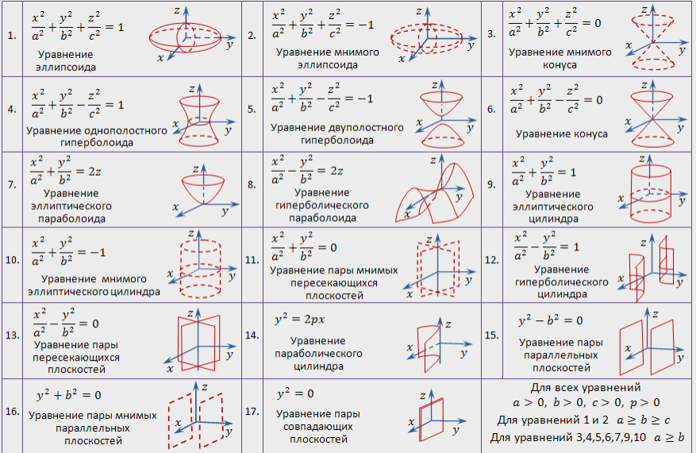
\includegraphics[height=6cm,width=1\textwidth,keepaspectratio]{curve_eq_rus.png}
            \label{fig:curve_eq_rus.png}
        \end{figure}
    \end{frame}

\begin{frame}[t]{Generator}
\framesubtitle{Definition}
\begin{columns}[T,onlytextwidth]
    \begin{column}{0.49\textwidth}
        A line all points of which lie on a quadric is called \textbf{a generator of the quadric}. An elliptic cone is a quadric surface which is generated by a straight line which passes through a fixed point and which intersect an ellipse. Then, the equation of generator is:
\begin{align*}
    \frac{x-x_v}{l} = \frac{y-y_v}{m} = \frac{z-z_v}{n}
\end{align*}
    \end{column}
    \begin{column}{0.49\textwidth}
        \vspace{-0.6cm}
        \begin{figure}[H]
            \centering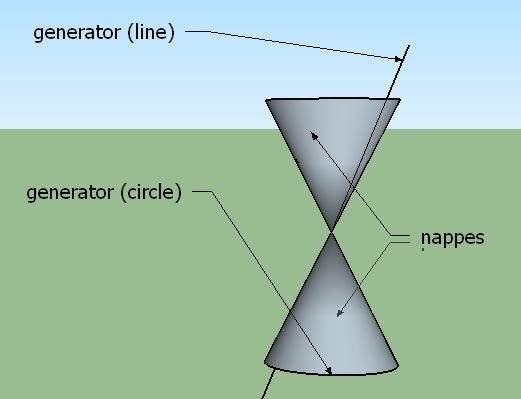
\includegraphics[height=6cm,width=1\textwidth,keepaspectratio]{generators.jpg}
            % \caption{caption_name}
            \label{fig:generators.jpg}
        \end{figure}
    \end{column}
\end{columns}

\end{frame}

\begin{frame}[t]{Task 1}
    \framesubtitle{}
    \only<1>{
        Find the equation of the cone with its vertex at $(1,1,1)$ and which passes through the curve $x^2+y^2=4, z =2$.}
    \only<2>{
        \alert{\Large Answer}
        \scriptsize
        \begin{columns}[T,onlytextwidth]
            \begin{column}{0.49\textwidth}
                Let's find a generator of the cone, when $V(1, 1, 1)$. Also, let's consider that our line intersects the plane $z = 2$:
                \begin{align}
                    \frac{x-1}{l} = \frac{y-1}{m} = \frac{1}{n}, \Rightarrow 
                    x = \frac{l}{n} + 1,~y = \frac{m}{n} + 1
                \end{align}
                This point lies on the curve $x^2+y^2=4$, hence -- put (1) into the circle  
                \begin{align}
                    \left(\frac{l}{n} + 1\right)^2 + \left(\frac{m}{n} + 1\right)^2 = 4
                \end{align}
                Our goal to eliminate $l,\ m,\ n$ from equation above.
                \begin{align*}
                    \frac{l}{n} = \frac{x-1}{z-1},~\frac{m}{n} = \frac{y-1}{z-1} \rightarrow \text{(2)} \\
                    \left(\frac{x-1}{z-1} + 1\right)^2 + \left(\frac{y-1}{z-1} + 1\right)^2 = 4 \text{ after simplification} \Rightarrow \\
                    \Rightarrow x^2 + y^2 - 2z^2 + 2xz + 2yz - 4x - 4y + 4 = 0
                \end{align*}
            \end{column}
            \begin{column}{0.49\textwidth}
                \begin{figure}[H]
                    \href{https://www.geogebra.org/calculator/enfuyejs}{
                        \centering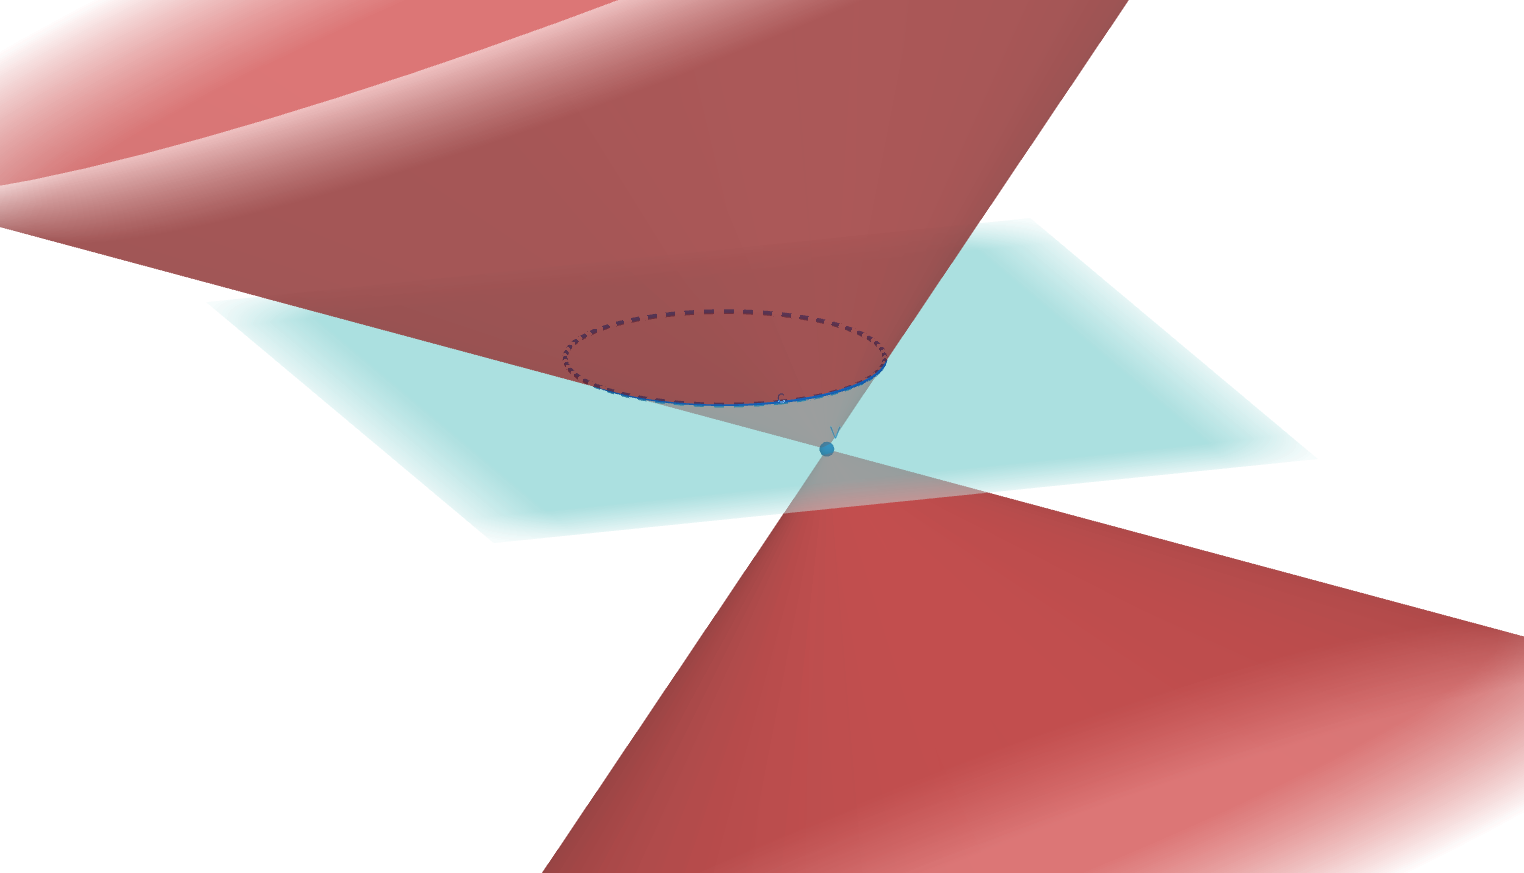
\includegraphics[height=6cm,width=1\textwidth,keepaspectratio]{1ans.png}}
                    \label{fig:1ans.png}
                \end{figure}
            \end{column}
        \end{columns}
    }
\end{frame}

\begin{frame}[t]{Task 2}
    \framesubtitle{}
    \only<1>{
        Find the equation of the cone with its vertex at the origin, which passes through the curve $ax^2+by^2+cz^2-1= 0 = \alpha x^2 - \beta y^2 - 2z$.}
    \only<2>{
        \alert{\Large Answer}
        \scriptsize
        \begin{multicols}{2}
            This task is an upgraded version on the 1-st task.

            Right now, we don't know neither the center of a given curve, nor the conic section passed through the center. Let's find it

            \begin{align*}
                ax^2 + by^2 + cz^2 - 1 - \alpha x^2 + \beta y^2 + 2 z = 0 \Rightarrow \\
                \Rightarrow (a-\alpha)x^2+(b+\beta)y^2+c(z+\frac{1}{c})^2=\frac{c+1}{c}
            \end{align*}

            The center of the curve is $(0,\ 0,\ =-\frac{1}{c})$. Let's find a conic section in a plane, perpendicular to $z$ axis (just simplification, can choose any).

            \begin{align}
                (a-\alpha)x^2+(b+\beta)y^2=\frac{c+1}{c}
            \end{align}

            Now, the task is the same as the first one. We know the vertex (origin) and a curve, which should be passed through.

            \begin{align*}
                \frac{x - 0}{l} = \frac{y - 0}{m} = \frac{-\frac{1}{c} - 0}{n}, \Rightarrow 
                x = -\frac{l}{cn},~y = -\frac{m}{cn}
            \end{align*}

            Put $x,\ y$ into (3):
            \begin{align}
                (a-\alpha)\frac{l^2}{c^2n^2} + (b+\beta)\frac{m^2}{c^2n^2}=\frac{c+1}{c}
            \end{align}
            Based on equation of generator we will receive $\frac{l}{n}=\frac{x}{z};\ \frac{m}{n}=\frac{y}{z}$. Put it into (4)
            \begin{align*} 
                (a-\alpha)\frac{x^2}{z^2} + (b+\beta)\frac{y^2}{z^2}=c^2+c \Rightarrow \\
                (a-\alpha)x^2+(b+\beta)y^2 - (c^2+c)z^2=0
            \end{align*}
        \end{multicols}
    }
\end{frame}

\begin{frame}[t]{Task 3}
    \framesubtitle{}
    \only<1>{
        Find the equation of the cone, which passes through the axes.}
    \only<2>{
        \alert{\Large Answer}
        \begin{figure}[H]
            \centering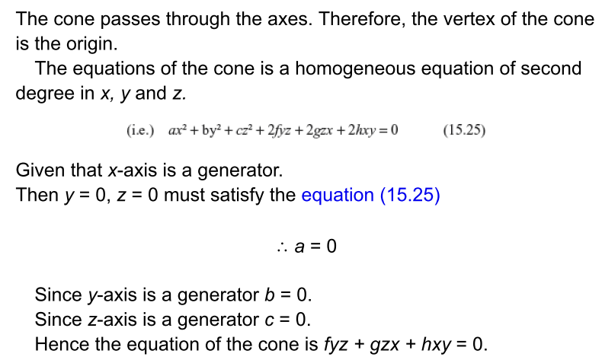
\includegraphics[height=5.5cm,width=1\textwidth,keepaspectratio]{3ans.png}
            % \caption{caption_name}
            \label{fig:3ans.png}
        \end{figure}
    }
\end{frame}

\begin{frame}[t]{Task 4}
    \framesubtitle{}
    \only<1>{
        Find the equation of the right circular cone whose vertex is at the origin, whose axis is the line $\dfrac{x}{1}=\dfrac{y}{2}=\dfrac{z}{3}$ and which has a vertical angle of $60^\circ$.}
    \only<2>{
        \alert{\Large Answer}
        \begin{figure}[H]
            \centering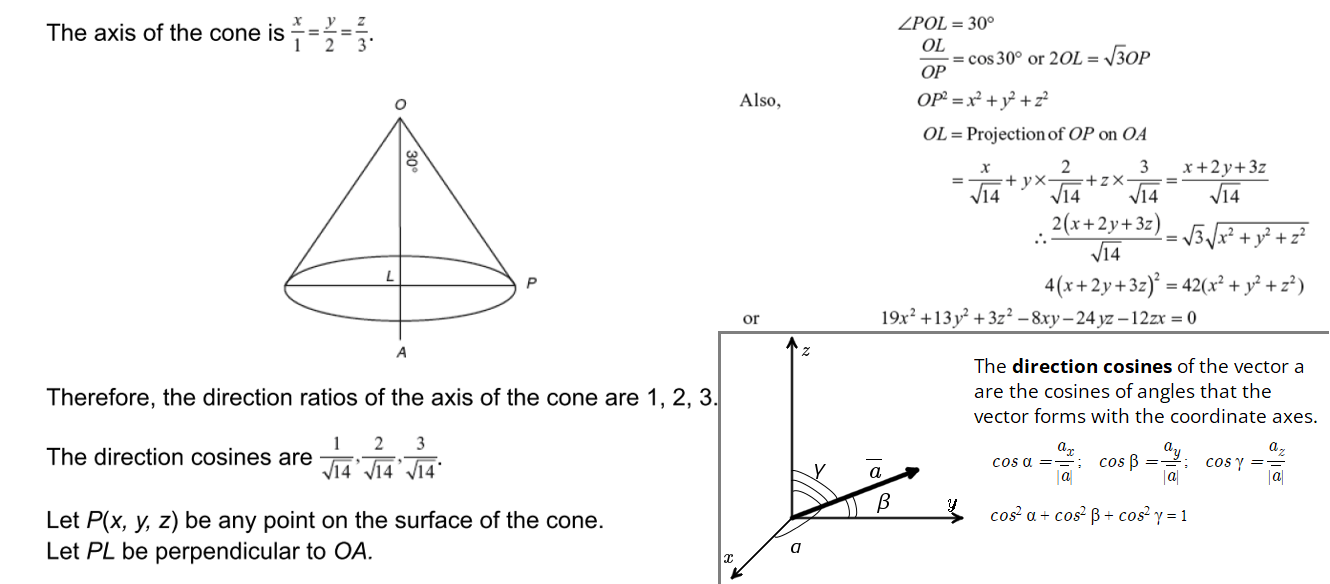
\includegraphics[height=5.5cm,width=1\textwidth,keepaspectratio]{4ans.png}
            % \caption{caption_name}
            \label{fig:4ans.png}
        \end{figure}
    }
\end{frame}

\begin{frame}[t]{Task 5}
    \framesubtitle{}
    \only<1>{
        Find the equation of the cylinder whose generators are parallel to the line $\dfrac{x}{-1}=\dfrac{y}{2}=\dfrac{z}{3}$ and whose directional curve is $x^2+y^2=9, z=1$.}
    \only<2>{
        \alert{\Large Answer}
        \begin{figure}[H]
            \centering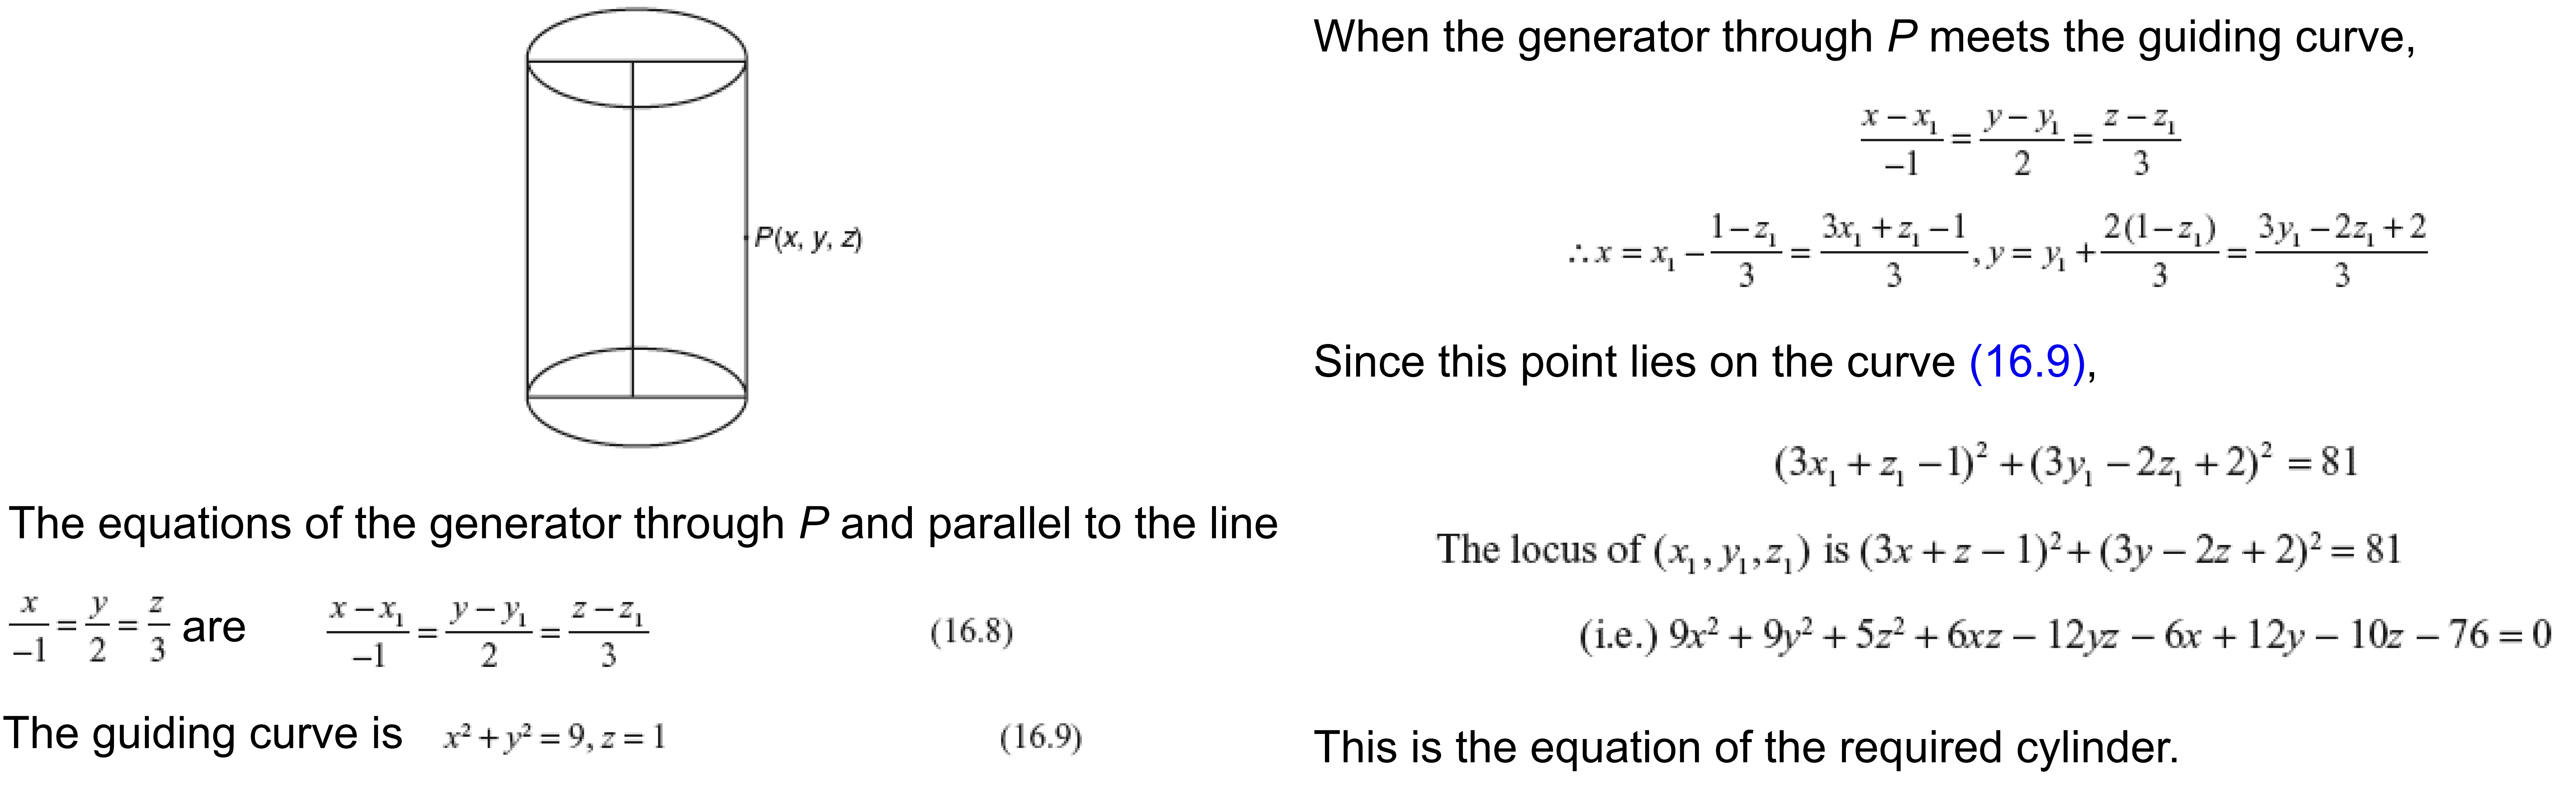
\includegraphics[height=5.5cm,width=1\textwidth,keepaspectratio]{5ans.png}
            % \caption{caption_name}
            \label{fig:5ans.png}
        \end{figure}
    }
\end{frame}

\begin{frame}[t]{Task 6}
    \framesubtitle{}
    \only<1>{
        Find the equations of the right circular cylinder of radius $3$ with equations of axis as  $\dfrac{x-1}{2}=\dfrac{y-3}{2}=\dfrac{z-5}{-1}$.}
    \only<2>{
        \alert{\Large Answer}
        \begin{figure}[H]
            \centering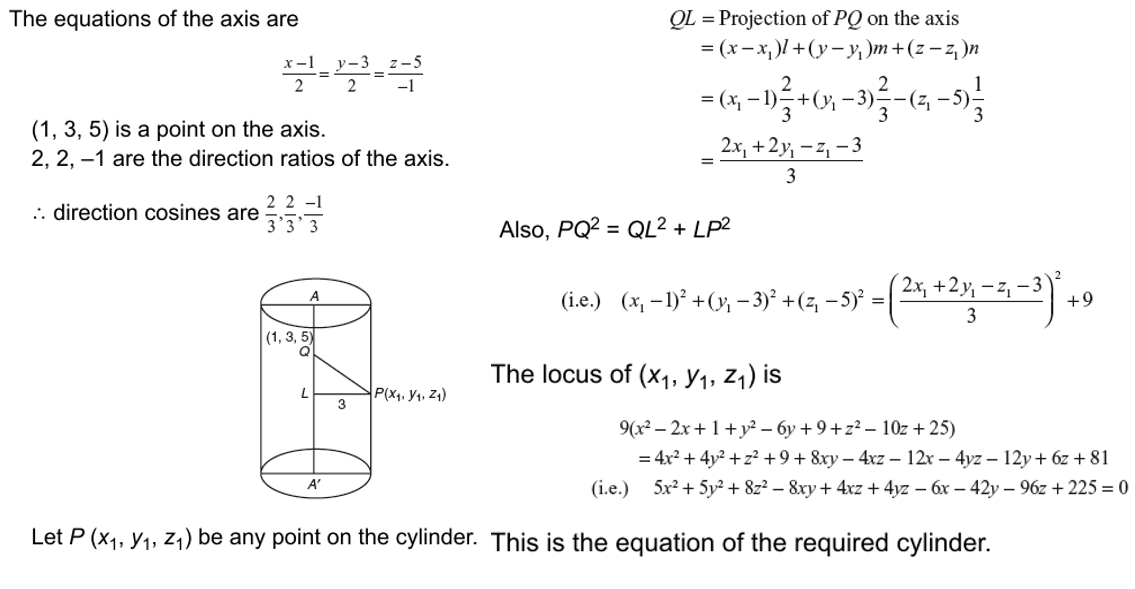
\includegraphics[height=5.5cm,width=1\textwidth,keepaspectratio]{6ans.png}
            % \caption{caption_name}
            \label{fig:6ans.png}
        \end{figure}
    }
\end{frame}

\begin{frame}[t]{Task 7}
    \framesubtitle{}
    \only<1>{
    Find the equation of the enveloping cylinder of the sphere $x^2+y^2+z^2-2x+4y=1$ having its generators parallel to the line $x=y=z$.
    % \vspace{-0.5cm}
    \begin{figure}[H]
        \centering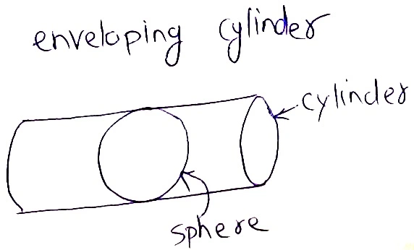
\includegraphics[height=4cm,width=1\textwidth,keepaspectratio]{7.png}
        % \caption{caption_name}
        \label{fig:7.png}
    \end{figure} }
    \only<2>{
        \alert{\Large Answer}
        \scriptsize
        \begin{columns}[T,onlytextwidth]
            \begin{column}{0.59\textwidth}
                Let $P(x_1,\ y_1,\ z_1)$ be any point on a tangent, which is parallel to the line $x=y=z$.

                Hence, the equation of the tangent lines are
                \begin{align} \label{eq:t7_1}
                    \dfrac{x-x_1}{1}=\dfrac{y-y_1}{1}=\dfrac{z-z_1}{1}
                \end{align}
                Any point on this line is $(x_1+\tau,\ y_1+\tau,\ z_1+\tau)$. This point lies in this sphere.
                \begin{align}
                    \label{eq:t7_2}
                    x^2+y^2+z^2-2x+4y-1=0
                \end{align}
                \begin{align*}
                    (x_1+\tau)^2+(y_1+\tau)^2+(z_1+\tau)^2-2(x_1+\tau)+4(y_1+\tau)-1=0 \Rightarrow \\ \Rightarrow  3\tau^2 + 2\tau(x_1+y_1+z_1+1) + (x_1^2+y_1^2+z_1^2-2x_1+4y_1-1)=0
                \end{align*}
                If (5) touches (6), $\tau$ is unique ($\mathcal{D} =0$).
                \begin{align}
                    \mathcal{D}= 4(x_1+y_1+z_1+1)^2-12(x_1^2+y_1^2+z_1^2-2x_1+4y_1-1)=0 
                \end{align}
                Solving (7) and change $P$ to general form, we are obtaining the answer
                \begin{align*}
                    x^2+y^2+5y +z^2 -4x -z -xy -xz -yz -2 =0 
                \end{align*}
                
            \end{column}
            \begin{column}{0.39\textwidth}
                \vspace{-0.6cm}
                \begin{figure}[H]
                    \href{https://www.geogebra.org/calculator/uqzwjqu6}{
                        \centering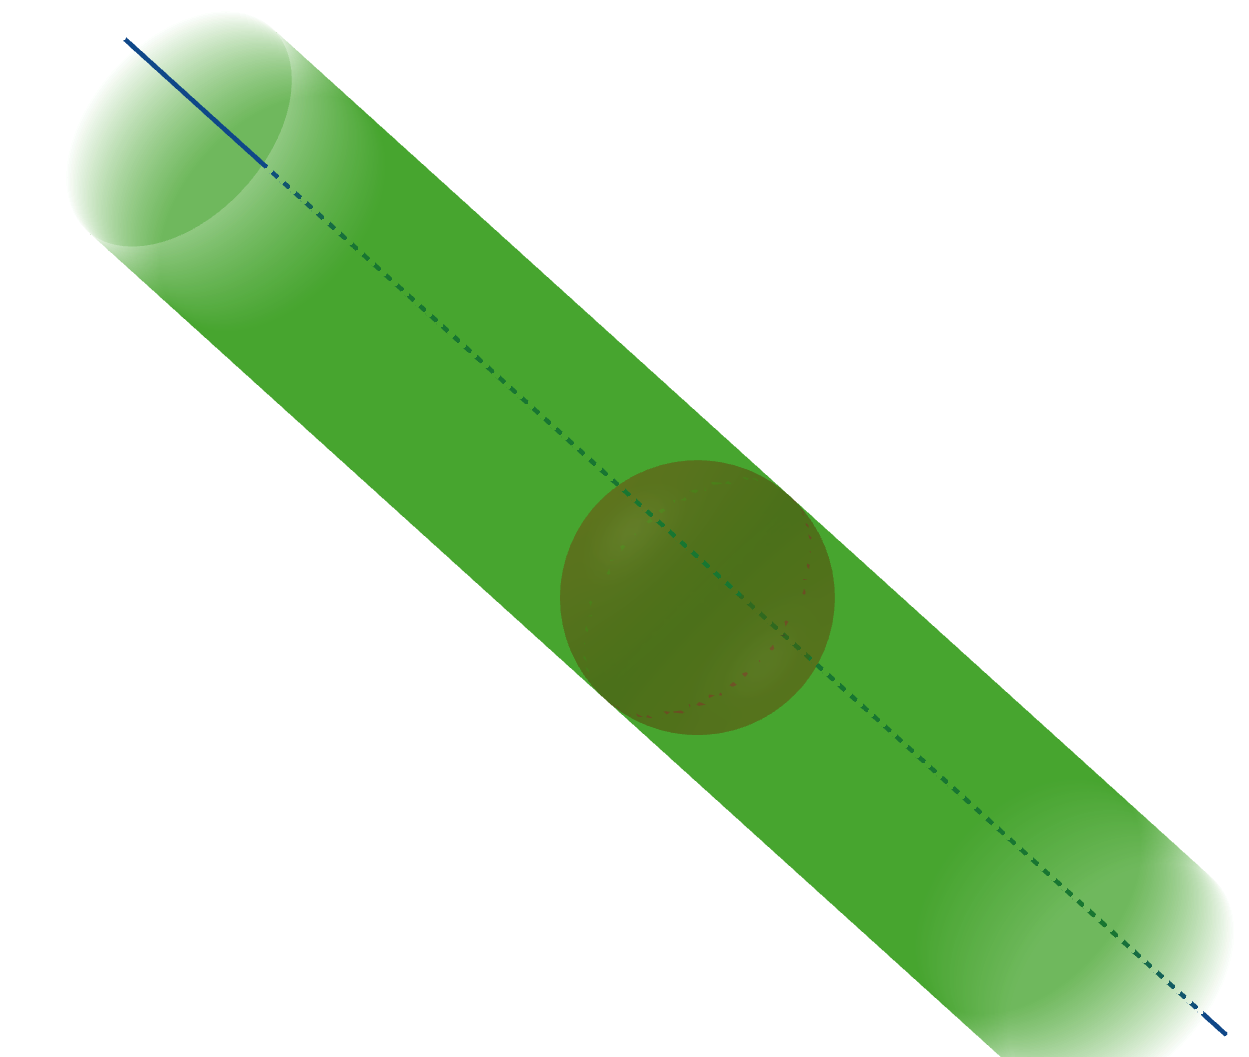
\includegraphics[height=6cm,width=1\textwidth,keepaspectratio]{7ans.png}}
                    \label{fig:7ans.png}
                \end{figure}
            \end{column}
        \end{columns}
    }
\end{frame}
\begin{frame}[t]{Reference material}
    \Large
    \begin{itemize}
        \item \href{https://onlinemschool.com/math/formula/cone/}{Cone, generatrix (OnlineMSchool)}
        \item \href{https://onlinemschool.com/math/library/vector/cos/}{Direction cosines (OnlineMSchool)}
    \end{itemize}
\end{frame}

\fbckg{fibeamer/figs/last_page.png}
\frame[plain]{}

\end{document}